\section{Teilbericht Fahrzeuge}

Ziel der Teilgruppe Fahrzeuge ist es, einen autonomen Transport zwischen den Rampen zu realisieren. Dafür sollen die Volksbots in der Lage sein, auf die eingehenden Aufträge zu reagieren.
Dies beinhaltet die Teilnahme an Auktionen ( Jobverteilung ), welche durch eine Aufwandsabschätzung des Auftrages eines jeden Volksbots entschieden werden. Nach der Zuweisung an den besten geeigneten Volksbot soll dieser das Paket von der entsprechenden Startrampe holen und zur Zielrampe transportieren.

Folgendes wird in den nächsten Unterkapiteln behandelt:

\begin{itemize}
	\item Anforderungskatalog an das Endsystem
	\item Beschreibung der Komponenten
	\item Werkzeuge
	\item Architektur
	\item Implementierung
	\item Erreichte Funktionalitäten
	\item Herausforderungen
	\item Ausblick
\end{itemize} 


\subsection{Anforderungen}
In diesem Abschnitt werden die gestellten Anforderungen zusammengetragen. Wir unterscheiden dabei zwischen funktionalen Anforderungen, die die direkte Funktionalität des fertigen Systems beschreiben, und nicht-funktionalen Anforderungen, die die qualitativen Eigenschaften des Systems widerspiegeln.
\subsubsection{Funktionale Anforderungen}
\begin{enumerate}
\item \textbf{Plattform}: Die physische Zelle wird als Netzwerk von Knoten in einem drahtlosen Sensornetzwerk implementiert. Als Plattform dienen MICAz-Module mit Atmel ATMega 128 Mikrocontroller und CC2420 Funkchip (siehe \autoref{MICAZ}).
 \item \textbf{Aktorik/Sensorik}: Die Rampen verfügen über Magnetstifte zum Vereinzeln der Pakete und Lichtschranken zum Erkennen von Paketen. Sie werden von den MICAz-Modulen angesteuert beziehungsweise ausgelesen.
 \item \textbf{Kommunikation}: Die MICAz-Module auf Rampen und Volksbots kommunizieren drahtlos untereinander auf Basis von Agenten-Nachrichten.
 \item \textbf{Synchronisation}: Die Simulation wird über ein Micaz-Modul, das als Gateway fungiert, an die drahtlose Kommunikation angebunden. Die Synchronisation der Zustände erfolgt über eine serielle Schnittstelle.
 \item \textbf{Disposition}: Die Controller kennen den Belegungszustand der Rampe und generieren nach dem FIFO-Prinzip Aufträge, die sie an die Volksbots vergeben.
 \item \textbf{Übergabe}: Wenn eine Ein- oder Auslagerung an einer Rampe ausgeführt werden soll, so übernimmt der Controller der Rampe die Kontrolle über die Fördereinheit des Fahrzeugs und sorgt dafür, dass das Paket verladen wird.
 \item \textbf{Kooperation}: Einsatz kooperativer Lösungsstrategien für die Materialflusssteuerung, Überwachung und Steuerung mittels Multi-Agentensystem.
\end{enumerate}

\subsubsection{Nicht-funktionale Anforderungen}
\begin{enumerate}
\item \textbf{Ressourcen}: Bei der Entwicklung muss 
auf den sparsamen Umgang mit Hardwareressourcen (Rechenzeit, Kommunikationsbandbreite, Speicher) geachtet werden. Insbesondere der vorhandene Arbeitsspeicher und das Kommunikationsmedium dürfen nicht überlastet werden, um einen stabilen Betrieb zu garantieren. 
\item \textbf{Stabilität}: Es müssen Maßnahmen getroffen werden, um ein stabiles System zu schaffen. Dies gilt insbesondere für die möglichst verlustfreie Übertragung von drahtlosen Nachrichten.
\item \textbf{Volksbots}: Die Module des Materialfluss über eine definierte Schnittstelle mit den Fahrzeugen kommunizieren, um auf die Aktorik und Sensorik der Volksbots zugreifen und schließlich einen Transport der Pakete gewährleisten zu können.
\end{enumerate}

\subsection{Beschreibung der Komponenten}
Dieser Abschnitt beschreibt die physikalischen Komponenten, die von der Teilgruppe Materialfluss verwendet wurden. Zu den diesen Komponenten zählen die Rampen, sowie die \textsc{Mica}z-Module mit ihren Mikrocontrollern. 
\subsubsection{Rampen}
Rampen stellen Ein- und Ausgänge, sowie Zwischenlager im physischen System dar. Auf einer Rampe finden bis zu vier Pakete Platz. Bolzen hinter dem ersten Paket, separiert dieses von den anderen Dreien. Damit das vorderste Paket nicht vorne von der Rampe herunterfällt, sind an der Vorderseite zwei weitere Bolzen angebracht. 

Durch vier Lichtschranken, wird eine Überwachung der Rampe ermöglicht. Diese beinhaltet zum einen das Abfragen, wie viele Pakete auf einer Rampe liegen. Zum anderen kann durch die Überwachung überprüft werden, an welcher Stelle Pakete liegen.

Alle vier Bolzen sind seitlich der Rampe befestigt. Eine autonome Steuerung der Rampen, wird durch ein angebrachtes \textsc{Mica}z-Modul ermöglicht.
\autoref{fig:skiram} zeigt ein Beispiel solch einer Rampe.

\begin{figure}[h!]
	\centering
		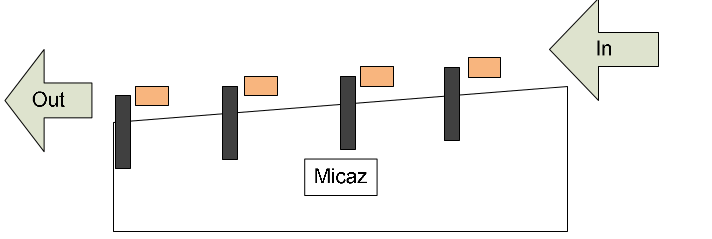
\includegraphics[width=0.9\textwidth]{SkizzeRampe.png}
	\caption{Beispiel einer eingesetzten Rampe}
	\label{fig:skiram}
\end{figure}

\subsubsection{Mikrocontroller}
Ein Mikrocontroller ist ein vollständiger Kleinstrechner auf einem einzigen Chip, dessen Zentraleinheit aus einem oder mehreren Mikroprozessen besteht. Zusätzlich enthält ein Mikrocontroller Speicher und Ein- bzw. Ausgabeschnittstellen zur Außenwelt. Dazu können neben einfach Ausgangspins auch komplexere Busprotokolle wie etwa USART, SPI oder CAN gehören.

Mikrocontroller werden eingesetzt, wenn eine Kommunikations- oder Steuerungsaufgabe mit möglichst geringen Ressourcen (Baugröße, Energie, Kosten) gelöst werden müssen. Die in einem Mikrocontroller verbauten Prozessorkern, Speicher und die Aus- und Eingabeschnittstellen, sind auf die Lösung derartiger Aufgaben zugeschnitten. Die große Anzahl an potenziellen Aufgabenstellungen hat zur Folge, dass es eine Vielfalt von Mikrocontrollern gibt. Meist sind die Mikrocontroller deshalb in Mikrocontrollerfamilien aufgeteilt. Innerhalb einer Familie unterscheiden sich die Controller nicht im Prozessorkern, sondern im verfügbaren Speicher und in den Ein- und Ausgabeschnittstellen \cite{ECHT2005}. In \autoref{fig:aufbmc} ist der schematische Aufbau eines MCs dargestellt.
\begin{figure}[th]
	\centering
		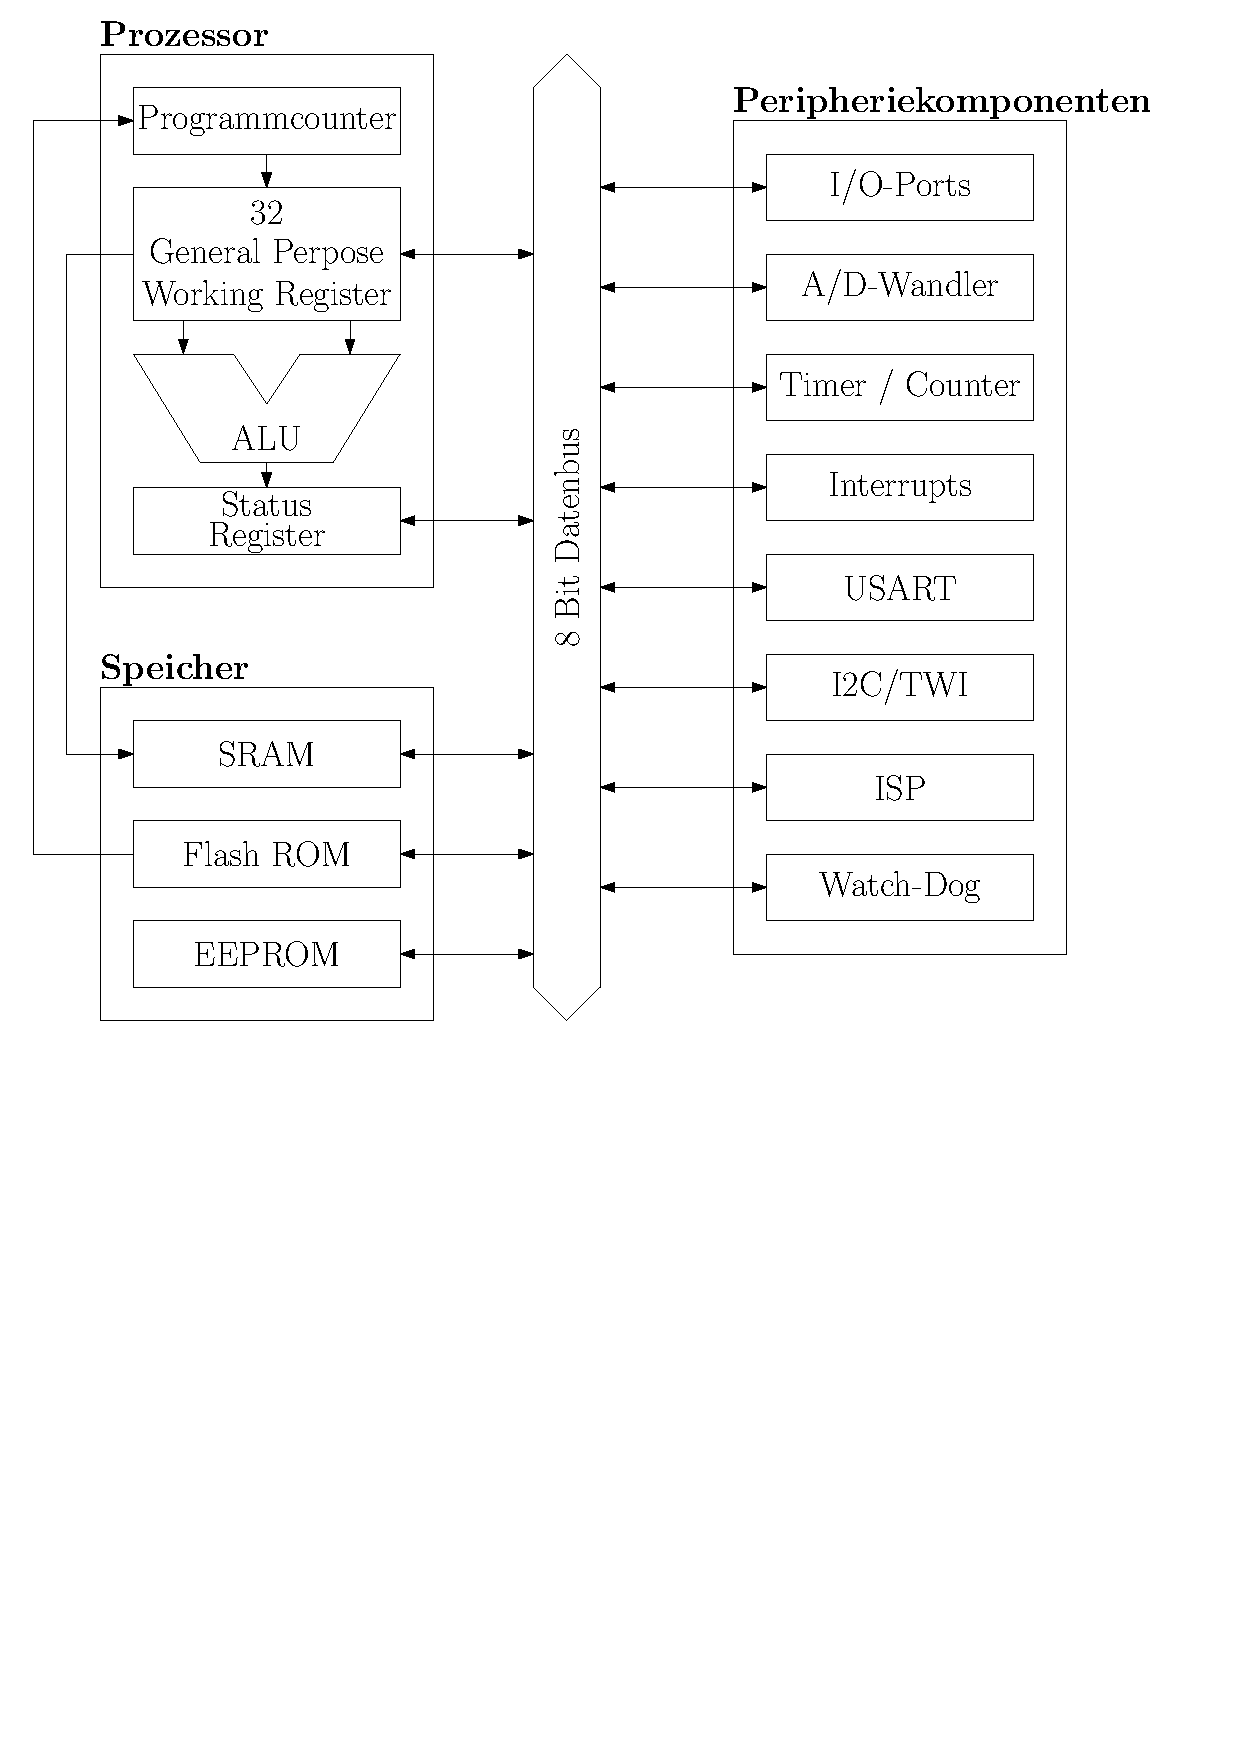
\includegraphics[width=0.8\textwidth]{flow/schemamc.pdf}
	\caption{Schematischer Aufbau eines Mikrocontrollers vgl. \cite{Brinkschulte:2002:Mikrocontroller}}
	\label{fig:aufbmc}
\end{figure}

Die zentrale Steuereinheit eines MCs ist der \textbf{Prozessor} (engl.: Central Processing Unit (CPU)). Sie ist die wichtigste Funktionseinheit und für die Verarbeitung von Befehlen und arithmetischen Berechnungen verantwortlich. Über den internen Bus kann die CPU mit weiteren Grundbausteien kommunizieren und beispielsweise auf Daten innerhalb des Speichers zugreifen.

Der \textbf{Speicher} besteht in der Regel aus dem Arbeitsspeicher (RAM, kurz für: Random Access Memory) und dem Programmspeicher bzw. Flash-Speicher. Normalerweise werden diese zwei Speichertypen logisch voneinander getrennt. Programme werden im nichtflüchtigen Flash-Speicher gesichert. Dieser kann mehrere Kilobyte (KB) bis Megabyte (MB) umfassen. Bei speziellen Systemen ist es möglich den Programmspeicher durch externe Flash-Komponenten zu erweitern um zusätzlichen Speicherplatz zu gewinnen.

Zwischenergebnisse, Messwerte von Sensoren, Steuergrößen usw. werden auf dem RAM abgelegt. Dieser ist deutlich schneller als der Flash-Speicher, verfügt aber in der Regel über deutlich weniger Speicherplatz. Alle Werte, welche zur Laufzeit im RAM abgelegt werden, sind im Gegensatz zum Flash-Speicher flüchtig. Das bedeutet, dass Daten bei einem Neustart des Mikrocontrollers nicht erhalten bleiben.

Durch die \textbf{Peripheriekomponenten} wird die Verbindung und Kommunikation zwischen Controller und Außenwelt ermöglicht. Über die digitalen Ein- und Ausgänge (GPIO, kurz für: General Purpose Input/Output) können Sensoren, Aktoren oder andere Systeme mit dem Mikrocontroller verbunden werden. Die meisten Mikrocontroller bieten eine Vielzahl von Ein- und Ausgängen \cite[S. 13-16]{SOM2012}.

Bei der Umsetzung des Projekts wurden \textsc{Mica}z-Module eingesetzt. Im Folgenden werden kurz die Eigenheiten dieser Module erläutert.

\paragraph{\textsc{Mica}z-Modul}
Ein \textsc{Mica}z-Modul ist drahtloser Sensornetzwerkknoten von der Firma Memsic. Mehrere dieser Module übernehmen in der physischen Zelle die Berechnung Geschäftslogik und die Steuerung der Rampen. \autoref{fig:micaz} zeigt ein solches Modul, während \autoref{fig:blockmicaz}  ein Blockdiagramm von dessen Struktur darstellt. Herzstück der Module ist ein ATMega128L-Mikrocontroller. Bei diesem handelt es sich um einen Low-Power-Mikrocontroller von der Firma Atmel. Darüber hinaus verfügt ein \textsc{Mica}z-Module über einen CC2420-Funkchip der Firma Texas Instruments. Dieser ermöglicht die drahtlose Kommunikation mit anderen Modulen auf einer Frequenz von 2.4 GHz ermöglicht. Es wird dabei der IEEE 802.15.4 Standard verwendet. Eine Antenne kann über eine MMCX-Schnittstelle mit dem Modul verbunden werden, um Signalstärke und -reichweite zu erhöhen. Weiter verfügen die Module über einen 128 KB großen Flash-Speicher.
Zugang zu einee Vielzahl der Leitungen des Moduls gewährt ein 51-poliger Steckverbinder. Über eine Erweiterungsplatine werden so etwa die Lichtschranken und Magnetbolzen der Rampe angeschlossen. Denkbar wäre auch ein größerer Arbeitsspeicher, alle nötigen Pins des Mikrocontrollers sind über den Steckverbinder erreichbar.
Im Projekt wurde die Steckverbindung weiterhin dafür genutzt, die \textsc{Mica}z-Module über ein \textsc{Mib}520 an einen PC anzuschließen, um sie über eine UART-Schnittstelle auszulesen und per JTAG (siehe \autoref{sec:JTAGICE3}) zu programmieren \cite{MICSHEET,C2420SHEET}.

\begin{figure}[th]
  \centering
    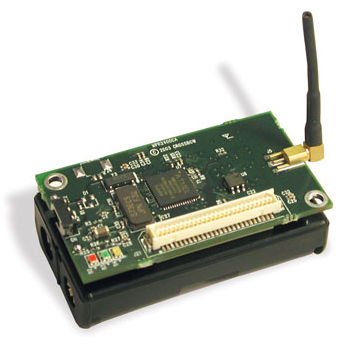
\includegraphics[width = 0.4\textwidth]{flow/micaz.png}
    \caption{\textsc{Mica}z-Modul \cite{Memsic:2014:Online}}
    \label{fig:micaz}
\end{figure}

\begin{figure}[th]
  \centering
    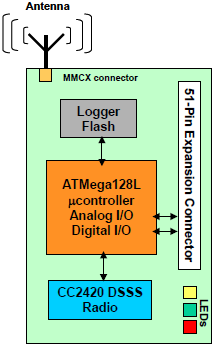
\includegraphics[width = 0.4\textwidth]{flow/blockmicaz.PNG}
    \caption{Blockdiagramm der \textsc{Mica}z-Module  \cite{Memsic:2014:Online}}
    \label{fig:blockmicaz}
\end{figure}

\paragraph{\textsc{Mib}520}
Ein \textsc{Mib}520 stellt eine Schnittstelle für \textsc{Mica}z-Module dar. Es erlaubt die Verbindung eines \textsc{Mica}z-Moduls mit einem Computer per USB-Schnittstelle. So kann über die USART-Schnittstelle des Moduls mit dem PC kommuniziert werden. Über diese Verbindung wurde die Schnittstelle zu den Volksbots realisiert. Weiterhin verfügt ein \textsc{Mib}520-Gateway über eine \textbf{JTAG}-Schnittstelle.


\subsection{Werkzeuge}

\subsubsection{Robot Operating System (ROS)}

Es gibt viele Robotik-Frameworks, die spezifisch für präzise Anwendungen, für Prototypen,
erstellt wurden. ROS strebt da eher das Allgemeine an. Das »Robot Operating System«
(ROS) ist ein Open-Source Framework für individuelle Roboter, das sich in der
Robotikforschung in den letzten Jahren etabliert hat und ein großes Repertoire an Software-Komponenten und -Werkzeugen für Robotikapplikationen bietet.\\
Die Entwicklung begann 2007 am Stanford Artificial Intelligence Laboratory im Rahmen des
Stanford-AI-Robot-Projektes (STAIR). Heute wird es hauptsächlich am Robotik Institut Willow
Garage weiterentwickelt. Seit April 2012 wird ROS von der neu gegründeten,
gemeinnützigen Organisation Open Source Robotics Foundation (OSRF) unterstützt. Die
Bibliotheken von ROS setzen auf Betriebssysteme wie Linux, Mac OS X oder Windows auf.
ROS ist nicht von einer spezifischen Sprache abhängig. Heutzutage gibt es 3 Grundlibraries
für ROS, die jeweils auf Python, Lisp und C++ ausgerichtet sind. Zwei Exmperimentier-
Librairies sind für Java und Lua erhältlich.
\subsubsection*{Was will ROS?}
\begin{itemize}
 \item ROS will unterstützen, Code für Forschung und Entwicklung wiederzuverwenden
 \item loser Verbund von individuellen Programmteilen (Nodes)
 \item einzelne Programmteile können einfach geteilt und verbreitet werden (Packages und Stacks)
 \item ROS stellt Repositories zu Verfügung, um dort Code zu teilen \cite{ROS:2014:Online}
(http://www.ros.org/browse)
\end{itemize}
\subsubsection*{Was kann ROS?}
Die Hauptbestandteile und Hauptaufgaben von ROS sind Hardwareabstraktion; Gerätetreiber; Implementierung 
von viel genutzten Funktionalitäten; Inter-Prozess-Kommunikation; Paket-Management
\subsubsection*{Aufgaben des ROS}
\begin{itemize}
 \item Interprozesskommunikation (IPC)
 \begin{itemize}
\item Problematik der Kommunikation zwischen verschiedenen Systemen des Roboters
\item Sicherheitseinstellung bei der Übertragung
\item Anforderung an die Geschwindigkeit / Schnelligkeit der Kommunikation
\item Koordination von Nachrichten durch zentralen Master
\end{itemize}
\item Paketverwaltung – Packages
\begin{itemize}
 \item ROS ist durch Softwarepakete (sogn. Packages) aufgebaut
 \item Ein Package beinhaltet Laufzeitprozesse (Nodes); ROS abhängige Bibliotheken;
Datensätze; Konfigurationsdateien;3rd Party Software
 \item Packages sind dazu, da um Code wiederverwendbar zu machen
\end{itemize}
\item Paketverwaltung – Stacks
\begin{itemize}
\item Sammlung von Paketen (Packages)
\item Der Sinn ist, dass Stacks die Verteilung und Verwendbarkeit von Code
vereinfachen
\item Meist viele Packages ähnlicher Aufgaben in einem Stack verpackt
\end{itemize}
\item Message (msg)
\begin{itemize}
 \item  Messages werden verwendet um unter ROS Nachrichten zwischen Knoten und
Topics auszutuaschen
\item Dafür verwendet ROS eine einfache Beschreibung der Datentypen in Textdateien
\item Durch diese Beschreibung kann für unterschiedliche Sprachen Code autogeneriert
werden
\item Diese sind in .msg-Dateien im msg- Unterverzeichnis eines ROS-Pakets abgelegt
\item Eigene Message-Typen sind mit Paket Ressource-Namen bezeichnet
\item Standard Messages sind mit std\_msg/msg/String.msg bezeichnet
\end{itemize}
\item Service
\begin{itemize}
 \item ROS verwendet eine eigene vereinfachte Service Description Language ("srv") für die
Beschreibung von ROS Service-Typen
\item Setzt direkt auf die ROS msg-Format auf
\item Ermöglicht die Anfrage / Antwort-Kommunikation zwischen den Knoten
\item Service-Beschreibungen sind in .srv-Dateien im srv- Unterverzeichnis eines Pakets
gespeichert
\item Service-Beschreibungen werden für die Verwendung mit dem Paket Ressource-
Namen bezeichnet
\item Z. B.: wird die Datei robot\_srvs/srv/SetJointCmd.srv als Service
robot\_srvs/SetJointCmd bezeichnet
\end{itemize}
\item Notes
\begin{itemize}
 \item Der Nachrichtenaustausch findet bei Nodes durch 3 Möglichkeiten statt: Parameter
Server;Topics; Services
\item Nodes werden wie in einem Graph angeordnet
\item In einem System laufen viele Nodes Parallel
\item Diese werden zu Beginn gestartet
\item Beispiele sind Nodes für: Laserscanner; Kinect; Pfadplanung
\end{itemize}
\item Topica
\begin{itemize}
 \item Topics verhalten sich wie ein virtuelles BUS-System Nodes können von Topics lesen
(subscribe)
\item Nodes können an Topics senden (publish)
\item Es gibt keine Begrenzung wie viele Nodes publsih oder subscribe auf ein Topic
machen
\end{itemize}
\end{itemize}
\subsubsection*{ROS-Datensystem}
ROS-Ressourcen sind in rangmäßiger Gliederung eingeordnet. Zwei Konzepte sind zu
verstehen:
\begin{itemize}
\item \textbf{Le package}: Es handelt sich hier um die Zentraleinheit der Softwareorganisation von
ROS. Ein Package ist ein Verzeichnis der die Knoten beinhaltet (wir werden hier
unten erklären, was ein Knoten ist) sowie die externen Librairies, Daten und XML
Konfigurationsdateien die manifest.xml genannt wird.
\item \textbf{Stack}: Stack bezeichnet eine Sammlung von Packagen. Sie ermöglicht mehrere
Funktionen wie Navigation, Lokalisierung und viele mehr. Ein Stack beinhaltet
mehrere Verzeichnisse sowie eine Konfigurationsdatei die stack.xml genannt wird.
\begin{itemize}
\item Vorhandene wichtige Stacks
\begin{itemize}
\item TF – Koordinatentransformation
\item Navigationstack
\item URDF - Modelle
\end{itemize}
\begin{itemize}
\item Beispiel Navigationstack
\begin{itemize}
\item Wertet Sensordaten aus z.B.: Laserdaten
\item Baut daraus mit gmapping (ebenfalls ein ROS-Stack) eine Begehbarkeitskarte
\item Warum? Zur Kollisionsvermeidung
\item Bei erfolgreicher Erstellung einer Map kann dann ein Ziel übergeben werde (Pfadplanung durch Navigationstack,
Kollisionsvermeidung, Reaktion auf sich ändernde Umgebung, Aufbau einer globalen Karte)
\end{itemize}
\end{itemize}
\end{itemize}
\end{itemize}
\subsubsection*{Vorteile und Nachteile des ROS}
\paragraph*{Vorteile}
\begin{itemize}
 \item Nachrichten-basierte Software Architektur
\begin{itemize}
\item Verschiedene Komponenten sind unabhängig voneinander mit dem System verbunden
\item Unterschiedliche Komponenten können miteinander verbunden werden, ohne jedes Mal das Programm neu zu Kompilieren
\item Netzwerkfähigkeit
\item Einfaches Debugging und Simulieren
\end{itemize}
\item Absturz eines Nodes führt nicht zum Absturz des ganzen
Systems
\item Für ROS lässt sich in mehreren Sprachen programmieren
\item ROS hat eine große Community, die viele Daten und Programme zu Verfügung
stellen
\end{itemize}
\paragraph*{Nachteile}
\begin{itemize}
 \item Durch Nachrichten-basierte Systemarchitektur Bottleneck bei großer Datenmenge
\item Steuerung des Systems über Kommandozeile
\end{itemize}

\subsubsection{Epos Control}

\subsubsection{SOPAS Engineeringtool}

Bei SOPAS ET handelt es sich um ein Entwicklungsprogramm von Sick. Dieses wird zur Ansteuerung und Konfiguration der Laserscanner und Hallsensosren verwendet.

\begin{itemize}
\item \textbf{ Erster Start }

Beim ausführen von SOPAS wird ein neues Projekt erstellt, in dem man die gewünschte Hardware selektiert und einbindet. Die Wahl der Hardware erfolgt hierbei über den Netzwerkscanassistenten oder manuell über den Gerätekatalog. Sobald die Kommunikation mit der Hardware aktiv ist, kann diese angesteuert werden. Änderungen der Konfiguration der Hardware sind im Projektbaum möglich oder sogar notwendig ( siehe Kapitel 7.7 Herausforderungen).
\end{itemize}


\subsection{Architektur}

Der systematische Aufbau des Volksbots ist in Abbildung \ref{fig:architecture_volksbot} dargestellt. Die Funktionen des Roboters basieren auf der Auswertung und Ansteuerung der Sensoren bzw. Aktoren. Alle Operationen, wie z.B. die Lokalisation, die Routenplanung, der Vorgang der Paketübergabe, laufen auf dem Robot Operating System und nutzen die Daten der Sensorik zur geeigneten Ansteuerung der Aktoren. Gesteuert werden die Operationen über die externe Kommunikationsebene, welche aus einem MICAz-Modul besteht. Hier werden Aufträge empfangen und auf der Operationsebene in zugehörige Ziele übersetzt.

\begin{figure}[h!]
 \centering
		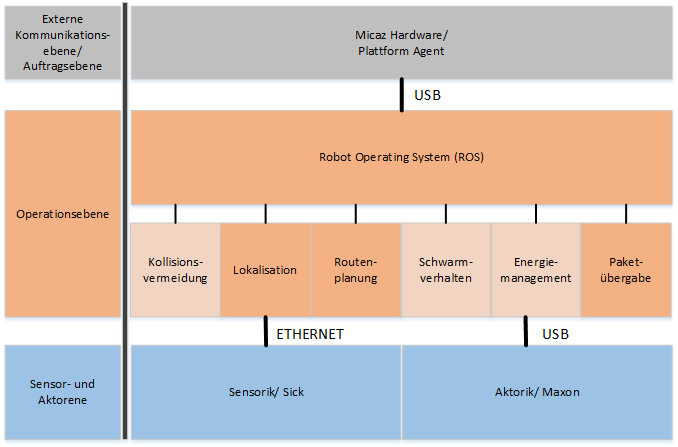
\includegraphics[width=1\textwidth]{drive/DRIVE_Architektur.png}
	\caption{Architektur des Volksbot}
	\label{fig:architecture_volksbot}
\end{figure}

Die in dunkleren rot hervorgehobenen Funktionen der Operationsebene deuten deren höhere Wichtigkeit an und geben ein erstes Anzeichen darauf welche Funktionen erfolgreich umgesetzt werden konnten.

\section{Implementierung}

Der erste Teil der Implementierung sah die Bereitstellung von Treibern für die komplette Hardware des Volksbots vor. Die Initialisierung und Ansteuerung der an den EPOS2-Controllern angeschlossenen Peripherie erfolgte unter der Verwendung der EPOS2 Bibliothek. Diese Bibliothek verfügt über alle benötigten Funktionen zum Ansteuern und Auslesen der Motoren und Lichtschranken, welche mit den EPOS-Controllern verbunden sind. Die Funktionen wurden dem ROS-Package „epos2-control“ zusammengeführt und sind in der Epos2MotorController-Node des Packages enthalten. 
Die Verwendung der Laserscanner, welche nicht mit den EPOS2-Controllern verbunden sind, wurde durch die Implementierung und Parametrisierung von im ROS vorhandenen Treibern gewährleistet. Dem an der Front des Roboters angebrachten SICK LMS100 Laserscanner, wurde dafür unter Windows eine feste IP-Adresse zugeordnet. Mit Hilfe dieser bekannten Adresse, konnte auch unter Ubuntu die Verbindung über Ethernet mit dem Laserscanner durch das Package „LMS1xx“  hergestellt werden.


\subsubsection{Implementierung der Navigation}
Nach erfolgreicher Inbetriebnahme der Hardware des Volksbots wurde die Odometrieberechnung anhand der zurückgelegten Strecke der Räder implementiert. Die Berechnung der zurückgelegten Wegstrecke und der Drehung des Roboters erfolgt über folgende Formeln\cite[S. 1]{Der:2000}:

\begin{equation}
\triangle s = \dfrac{\triangle R + \triangle L}{2}
\end{equation}
 
\begin{equation}
\triangle \alpha = \dfrac{\triangle R - \triangle L}{D}
\end{equation} 

Die Daten der Wegstrecke und der Drehung des Roboters werden genutzt, um mit folgenden Formeln die x- und y-Position des Roboters zu berechnen:

\begin{equation}
x = x(t-1) + (\triangle s * \cos (\alpha (t-1) + \triangle \alpha))
\end{equation} 

\begin{equation}
y = y(t-1) + (\triangle s * \sin (\alpha (t-1) + \triangle \alpha))
\end{equation} 

Der Drehwinkel des Roboters ergibt sich aus der Addition des vorherigen Winkels mit der zuletzt durchgeführten Änderung des Drehwinkels.

\lstinputlisting[language=C++, style=customc, captionpos=b, caption={Implementation der Odometrieberechnung}, label=lst:odom]{src/drive/lst/Odometrie.cpp}

Die Daten der Odometrie werden zur Lokalisierung des Roboters innerhalb einer mit dem SICK LMS100 Laserscanners erstellten Umgebungskarte verwendet. Die Implementierung erfolgte ebenso wie bei der Entwicklung der Treiber im „epos2-control“-Package. Bei der Erstellung der Umgebungskarte wurde auf das „Gmapping“-Package von ROS zurückgegriffen. Der darin enthaltene Algorithmus nutzt die Daten des Laserscanners, um während der Fahrt des Roboters aus seiner erfassten Umgebung eine Karte zu erstellen. Zur Visualisierung der Karte und der Daten des Laserscans wurde „Rviz“, ein Visualisierungstool innerhalb der ROS-Umgebung verwendet. Mit Hilfe von Rviz ist es neben der Visualisierung unter anderem möglich die initiale Position des Roboters, sowie Navigationsziele innerhalb der Karte festzulegen. (Screenshot Rviz) Mit dem Ziel den auftretenden Abweichungen der Odometrieberechnung entgegenzuwirken, wurde das „adaptive Monte Carlo Localisation“-Package (AMCL) implementiert. Vereinfacht formuliert, nutzt dieses Verfahren die Daten des Laserscans und der Karte, um mit Hilfe der Merkmale des aktuellen Scans und der zugrundeliegenden Daten der Kartenrepräsentation eine Schätzung der Position des Roboters auszuführen. \cite[S. 6]{Bischoff:2004}
Eine funktionsfähige Selbstlokalisation ist die Grundlage für eine erfolgreiche autonome Navigation in der Umgebung des Roboters. Das ROS-Framework stellt mit dem „move-base“-Package die nötigen Funktionen für die Navigation bereit. Das Package hat den Dijkstra-Algorithmus zur Wegplanung implementiert und nutzt zwei parametrisierbare Costmaps, um Eigenschaften wie z.B. den Mindestabstand zu Hindernissen oder das Verhalten bei Planungsfehlern festzulegen. Nach der Planung des Weges werden automatisch die passenden Steuerbefehle generiert. Falls der Volksbot in eine unvorhergesehene Situation gerät und seine geplante Route nicht mehr gültig ist, kommen Rettungs-Funktionen des Packages zum Einsatz. Dabei wird eine Rotation um die eigene Achse des Roboters durchgeführt, um einen geeigneten neuen Weg zu finden. 

\subsubsection{Implementierung der Paketübergabe}
Damit der Austausch der Pakete mit den Komponenten des Materialflusses erfolgen kann, musste die Kommunikation über die MICAz-Module und Automatismen zur Anpassung der Hub-Position an die Höhe der jeweiligen Rampe implementiert werden. Nachdem ein Auftrag vom Materialfluss empfangen wurde, wird die Annahme des Auftrags dem Materialfluss bestätigt und der Auftrag  in ein passendes Navigationsziel auf der Umgebungskarte umgesetzt.  Für den Prozess des Entschlüsselns von den Nachrichten des Materialflusses wurde ein ROS-Package namens „Simple-Navigation-Goals“ implementiert. Neben der Umsetzung von Navigationszielen sendet dieses Package ROS-interne Nachrichten, welche Informationen über die gewünschte Position des Hubs und das Erreichen der Zielposition enthalten.
Sobald die Zielposition erreicht wurde, beginnt die Hubsteuerung mit der Anpassung der Hubposition an die geforderte Höhe. Anschließend folgt eine Benachrichtigung an den Materialfluss und das Förderband wird in Gang gebracht. Die Auswertung der Lichtschranken bewirkt den Haltevorgang des Förderbands und das nächste Navigationsziel wird festgelegt.

\subsubsection{Struktur der einzelnen Funktionalitäten}



\begin{figure}[h!]
 \centering
		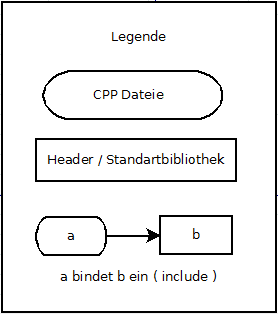
\includegraphics[width=0.4\textwidth]{drive/Legende.png}
	\caption{Legende zu Abb. 46 und 47}
	\label{fig:Legende}
\end{figure}

\begin{figure}[h!]
 \centering
		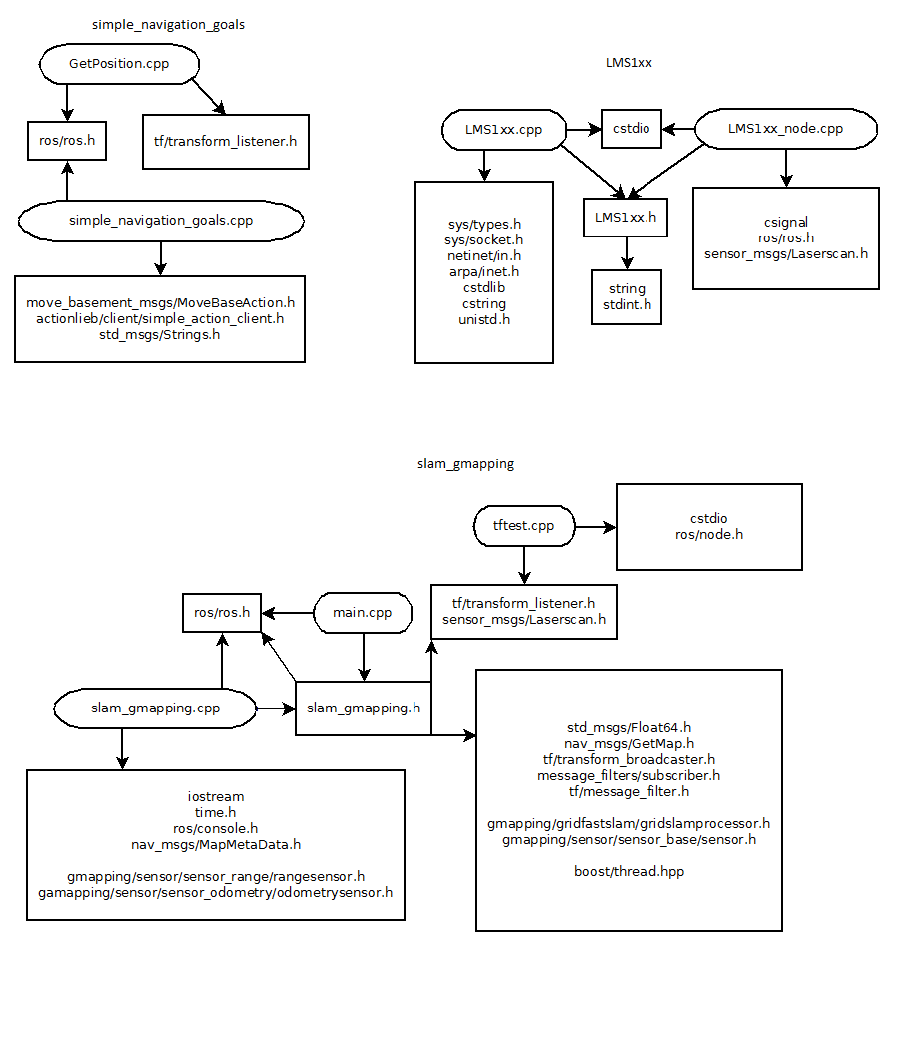
\includegraphics[width=1\textwidth]{drive/funktionen.png}
	\caption{eingebundene Funktionen in ROS}
	\label{fig:funktionen}
\end{figure}

\begin{figure}[h!]
 \centering
		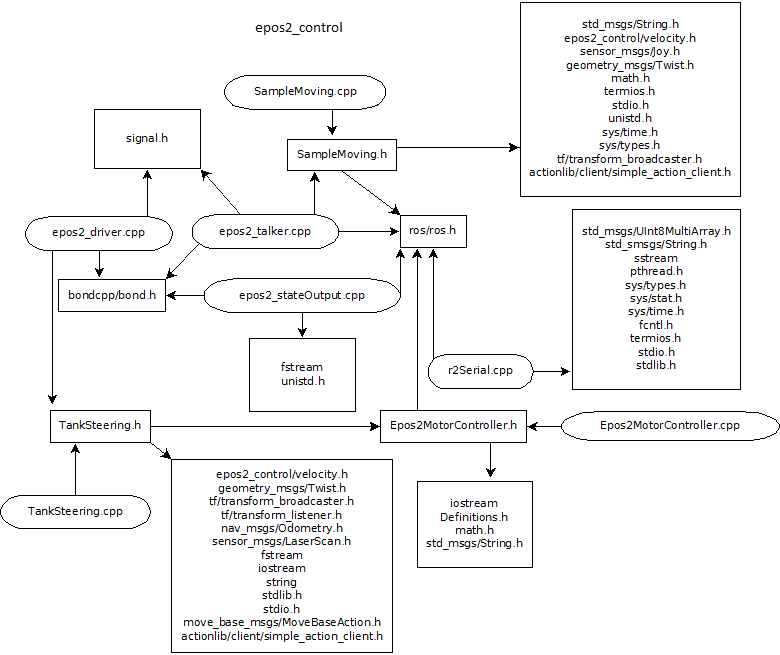
\includegraphics[width=1\textwidth]{drive/epos2_control.png}
	\caption{Hauptsteuerung des Systems ( Epos2 Control )}
	\label{fig:epos2_control}
\end{figure}


\input{src/drive/6_Funktionalitäten}

\subsection{Herausforderungen}

Bei der Implementierung der Funktionen des Volksbot traten einige Herausforderungen auf, deren Lösungen besonderen Aufwand hervorriefen oder nicht umgesetzt wurden. Ein Beispiel dafür ist die Selbstlokalisation des Roboters durch die Odometrieberechnung und dessen Verbesserung durch die adaptive Monte Carlo Lokalisation (AMCL). Aufgrund der Fehleranfälligkeit der einfachen Odometrie durch Einflüsse wie z.B. die Beschaffenheit des Bodens ist der Einsatz von Algorithmen wie die adaptive Monte Carlo Lokalisation, welcher die Daten des Laserscanners nutzt, notwendig.  Die Qualität der Odometrie musste durch das Kalibrieren des Parameters der Achsenlänge des Roboters erhöht werden, um die nötige Voraussetzung für einen funktionierenden AMCL-Algorithmus zu schaffen. Eine gute Odometrie lässt sich dadurch erkennen, dass die Punkte des Laserscans auch bei Bewegung weiterhin mit den Wänden der Umgebungskarte übereinstimmen. Getestet wurde die Odometrie durch die verzögerte Darstellung der Laserscans in Rviz bei der Drehung des Roboters. Die Laserscan-Punkte würden bei einer guten Odometrie den Raum relativ genau nachzeichnen und die Laserpunkte würden sich überlappen. Ein Vergleich zwischen einer guten Odometrie-Einstellung (links) und einer schlechten (rechts) ist in Abbildung \ref{fig:Odo_vergleich} dargestellt.

\begin{figure}[h!]
 \centering
		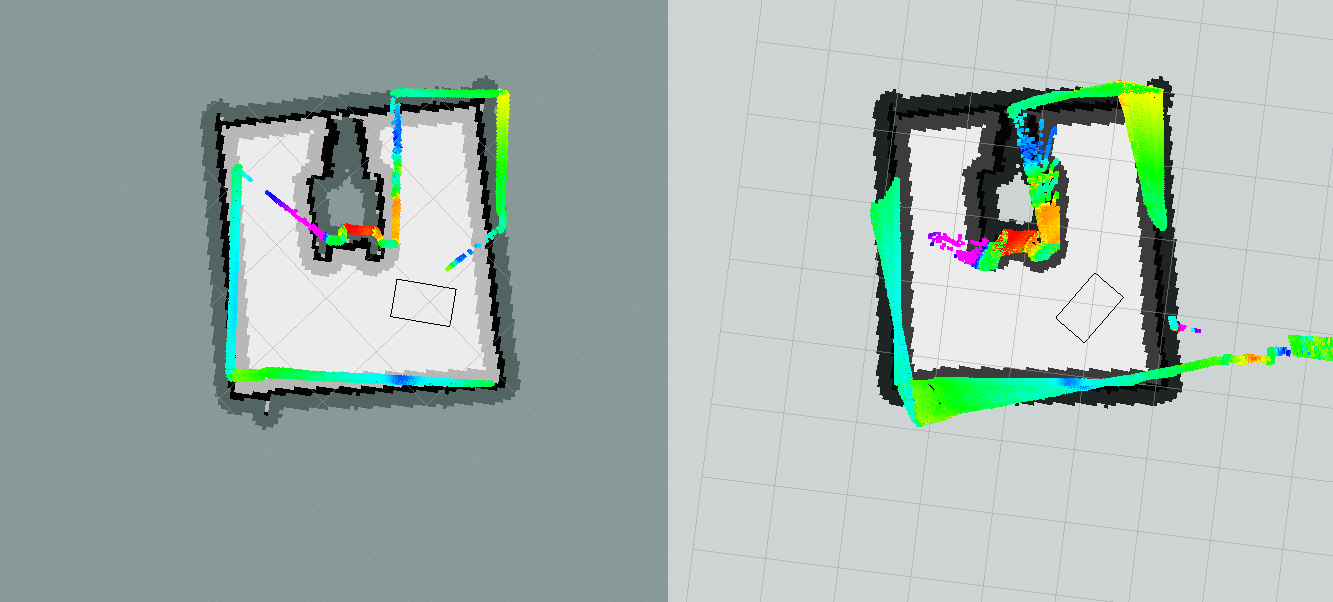
\includegraphics[width=1\textwidth]{drive/Odometrie_vergleich.png}
	\caption{Vergleich von Odometrie-Einstellungen mit Hilfe von verzögert dargestellten Laserscan-Punkten}
	\label{fig:Odo_vergleich}
\end{figure}

Bei der Parametrisierung der Wegplanung musste ein Gleichgewicht zwischen Geschwindigkeit und Genauigkeit gefunden werden, um ein stabiles System zu schaffen. Durch die Vielzahl der Möglichkeiten war die Suche nach geeigneten Einstellungen problematisch. Ein Beispiel dafür ist die Parametrisierung der Zieltoleranzen. Einerseits hat die Verringerung der Zieltoleranzen bewirkt, dass sich der Roboter der Zielposition exakter nähert. Andererseits dauert die Ausrichtung des Roboters deutlich länger, da der Roboter mehrere Rotationen ausführt bis die geeignete Position erreicht wurde. Letztlich wurde eine genauere Positionstreue des Roboters priorisiert, um die Fehleranfälligkeit bei der Paketübergabe zu senken.

Eine weitere Herausforderung stellte die Erkennung von Hindernissen dar, die ober- oder unterhalb des Laserscanners in den Raum ragen. Zur Lösung dieses Problems könnte ein weiterer bildgebender Sensor genutzt werden, um den gesamten Raum nach potenziellen Hindernissen zu untersuchen oder eine Anpassung der Arbeitsumgebung durchgeführt werden.

Mit großem Aufwand war die korrekte Ansteuerung der Maxon Controller verbunden. Besonders die Parametrisierung des kleineren Maxon Controllers unter ROS, welcher für den Betrieb des Förderbandes verwendet wird, stellte sich als Problem heraus. Schon kleinere Abweichungen der Parameter für Spannungs- und Beschleunigungswerte in der Ansteuerung des Controllers führten zu Systemabstürzen.
 
Die Programmierung und Parametrisierung der Teilfunktionen musste mit Blick auf
die CPU-Auslastung der Steuereinheit geschehen, da einige Berechnungen bei falscher
Verwendung zu sehr hohen Auslastungen und einer unzureichenden Performance des
Roboters führten. Ein Beispiel dafür ist die Funktion zur Kommunikation mit Hilfe des MICAz-Moduls, welche     regelmäßig unterbrochen werden musste.

Ein weiteres Problem stellte der LMS 100 Laserscanner von SICK dar. Dieser wird mittels Ethernet-Anschluss mit der Steuereinheit verbunden und sollte mittels seiner IP Adresse durch ROS direkt verwendet werden können. Allerdings konnte weder ROS noch SOPAS ET ( siehe Kapitel 3..3.3 ) auf den Scanner zugreifen. Beim erstellen eines Projekts in SOPAS war der Netzwerkscanassistent nicht in der Lage den Laserscanner zu erkennen und somit musste der LMS 100 manuell im Gerätekatalog ausgewählt und in das Projekt eingebunden werden. Bei der Verbindung zum LMS 100 wurde die bestehende IP Adresse des Scanners angezeigt und eine Neuzuweisung einer IP Adresse angeboten. Die Neuzuweisung der IP Adresse ist notwending, damit ROS eine Verbindung zum LMS 100 herstellen konnte.

\subsection{Ausblick}

Der Volksbot sollte um folgende Funktionalitäten erweitert werden:

\begin{itemize}

\item \textbf{Genauigkeit bei der Übergabe}: Die Genauigkeit des Heranfahrens an eine Zielposition, wie z.B. den Ausgang einer Rampe, muss verbessert werden, um eine erfolgreiche Übergabe zu gewährleisten. Durch die Fehleranfälligkeit der Odometrie sollte eine alternative Prozedur zur Ansteuerung der Rampen entwickelt werden, um die Paketübergabe mit höherer Erfolgswahrscheinlichkeit zu realisieren.

\item \textbf{Kollisionserkennung mobile Hindernisse - Schwarmverhalten}: Der Volksbot sollte Hindernisse, die sich selbstständig bewegen, erkennen und entsprechend reagieren. Dies könnte beim erkennen eines Objektes mittels einer Neuplanung der Route, einer kurzen Unterbrechung der Fahrt oder eines Ausweichmanövers umgesetzt werden. Besonders bei der Verwendung von mehreren Volksbots sollte eine Funktion zur Bahnreservierung implementiert werden. 

\item \textbf{Rückkopplung an Simulation}: Die Volksbots sollten ihre aktuelle Position, sowie den Beladungs- und Energiezustand an die Simulation zurückgeben.

\item \textbf{Fahralgorithmus}: Es können alternative Algorithmen implementiert werden, um die Berechnungszeiten zu verkürzen oder optimale Routen zu finden.

\item \textbf{Kostenabschätzung}: Eine optimale Berechnung zur Bestimmung der benötigten Zeit, Strecke und Energieverbrauchs würde die Jobverteilung effizienter gestalten.

\item \textbf{Ladestation}: Die Ladestation muss angebracht und getestet werde. Danach fehlt die automatische Erkennung des kritischen Zustandes, sowie das selbstständige anfahren der Ladestation, damit der Akku geladen werden kann. Hierbei handelt es sich um einen Prototypen der noch getestet werden muss.

\end{itemize}



















